\documentclass[10pt]{article}
\usepackage[polish]{babel}
\usepackage[utf8]{inputenc}
\usepackage[T1]{fontenc}
\usepackage{graphicx}
\usepackage[export]{adjustbox}
\graphicspath{ {./images/} }
\usepackage{amsmath}
\usepackage{amsfonts}
\usepackage{amssymb}
\usepackage[version=4]{mhchem}
\usepackage{stmaryrd}

\title{Zadania - runda I }

\author{Oświadczenie\\
Niniejszym oświadczam, że jako uczestnik konkursu „OD SZKOLNIAKA DO ŻAKA" zorganizowanego przez Centrum Nauczania Matematyki i Kształcenia na Odległość Politechniki Gdańskiej, wyrażam zgodę na przetwarzanie moich danych osobowych w zakresie niezbędnym dla potrzeb niniejszego konkursu.\\
Przyjmuję do wiadomości, że moje dane osobowe będą wykorzystane zgodnie z ustawą z dnia 29 sierpnia 1997 r. o ochronie danych osobowych (Dz.U. z 2002 r. nr 101, poz. 926 ze zm.) dla celów przeprowadzenia w/w konkursu.\\
Jednocześnie oświadczam, że zostałem poinformowany o tym, że:\\
- Administratorem danych osobowych konkursu jest: Politechnika Gdańska z siedzibą przy ul. Gabriela Narutowicza 11/12; 80-233 Gdańsk\\
- Przysługuje mi prawo do wglądu do moich danych i żądania ich poprawienia.\\
- Dane będą przetwarzane dla realizacji konkursu.\\
- Podanie danych jest dobrowolne.\\
- Nie przewiduje się przekazywania danych.}
\date{}


\begin{document}
\maketitle
Zadanie 1. (5p.) Obwód trójkąta wynosi 18cm. Jakie są długości jego boków, jeżeli długości te są liczbami naturalnymi, oraz suma długości dwóch boków jest o 6 cm większa od długości trzeciego boku?

Zadanie 2. (5p.) Na poniższym rysunku widzimy kwadrat KLMN, trójkąt LOM i trapez POLK. Wiemy, że bok kwadratu ma 3 cm długości, pole trójkąta jest dwukrotnie większe niż pole kwadratu, natomiast pole trapezu jest trzy razy większe od pola kwadratu. Oblicz długość odcinka KP.\\
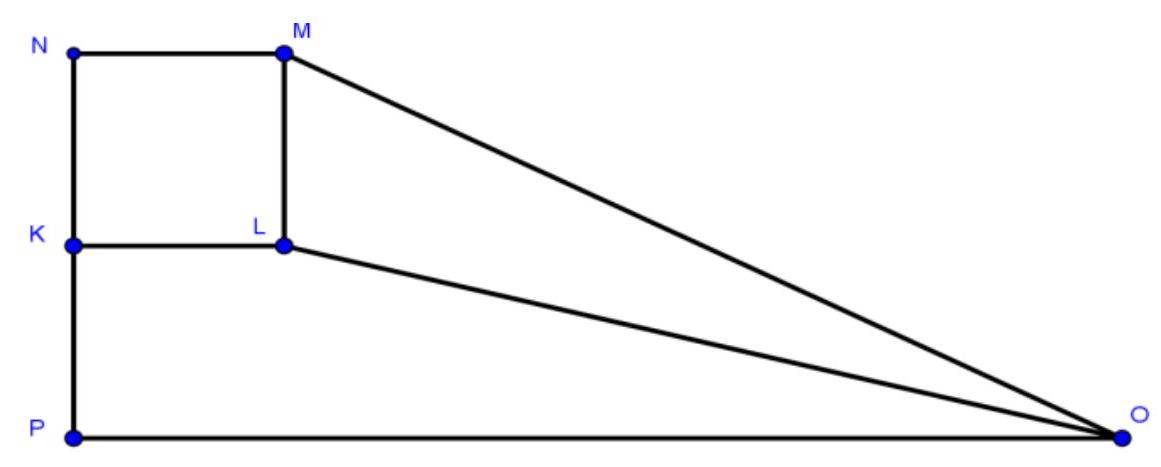
\includegraphics[max width=\textwidth, center]{2024_11_21_b991f37c2e98d6141e21g-1}

Zadanie 3. (5p.) Podaj największą i najmniejszą liczbę trzycyfrową, w których suma cyfr wynosi 21. lle wynosi różnica iloczynów cyfr tych liczb?

Zadanie 4. (6p.) Kwadrat rozcięto na 3 prostokąty dwoma prostymi równoległymi. Obwody tych prostokątów wynoszą odpowiednio: \(24 \mathrm{~cm}, 30 \mathrm{~cm}\) i 26 cm .\\
a). Ile wynosi długość boku kwadratu?\\
b). Oblicz pola tych prostokątów.

Zadanie 5. (5p.) Dane są dwie serie liczb tworzonych według pewnych regut:\\
seria 1: \(\quad 2,4,8,16,32, \ldots\);\\
seria 2: \(1,8,27,64,125, \ldots\).\\
Ile wynosi różnica dziesiątej liczby w serii 1-szej i dziesiątej liczby w serii 2-giej?\\
\(\qquad\)

\section*{ZAŁACZNIK DO KARTY UCZESTNIKA KONKURSU „OD SZKOLNIAKA DO ŻAKA" }
Wyrażam zgodę na uczestnictwo mojego dziecka w konkursie „OD SZKOLNIAKA DO ŻAKA"

Data r.\\
(podpis rodzica lub opiekuna prawnego ucznia)

\begin{abstract}
Akceptuję i wyrażam zgodę na postanowienia regulaminu konkursu „OD SZKOLNIAKA DO ŻAKA" zamieszczonego na stronie internetowej konkursu: http:/lpg.edu.pl/kursy-z-matematyki/o-konkursie
\end{abstract}

Data r.


\end{document}